\chapter{Zusammenbau der Hardware} \label{ch:ZusammenbauDrohne}
Der Zusammenbau einer Drohne erfordert Verständnis der einzelnen Komponenten und deren Integration zu einem funktionsfähigen System. Im Folgenden wird der Prozess des Zusammenbaus der Drohne in seinen wesentlichen Schritten beschrieben.

\section{Auswahl und Bestellen der Teile}
Die sorgfältige Selektion der Komponenten stellt einen wichitgen Schritt im Konstruktionsprozess der Drohne dar. Die Auswahl der Komponenten, wie beispielsweise Akkumulator, Motoren, Propeller, Flight Controller, Frame und Zubehör, erfolgt unter Berücksichtigung der spezifischen Anforderungen an die Drohne sowie ihrer geplanten Einsatzgebiete. Der Grund, weshalb hier eine klassische RC-Drohne zusammengebaut wurde, liegt in ihrer weiten Verbreitung. Dadurch steht eine breite Auswahl an Komponenten sowie detaillierte Beschreibungen und Dokumentationen zur Verfügung.

Der Selektionsprozess wurde in mehreren aufeinander aufbauenden Schritten durchgeführt. Zunächst wurden die Anforderungen an die Drohne definiert. Diese Anforderungen determinierten die notwendigen Merkmale der einzelnen Komponenten. In dieser Arbeit waren etwa eine hohe Leistungsfähigkeit der Motoren, ein leichtgewichtiger Frame sowie präzise Manöver von Bedeutung.
  
Die darauf folgende Recherche nach geeigneten Komponenten umfasste eine ausführliche Analyse von Bewertungen, Spezifikationen und Erfahrungsberichten aus Foren, Fachartikeln und YouTube-Videos, um die optimale Auswahl zu treffen. Im Anschluss wurden mehrere Optionen für jedes Bauteil hinsichtlich Preis, Leistung, Kompatibilität und Verfügbarkeit verglichen. Die finale Auswahl erfolgte unter Berücksichtigung des Projektbudgets, um die Balance zwischen Qualität und Kosten zu wahren. Nach erfolgter Entscheidung wurden die benötigten Teile (\autoref{sec:Teile}) bei den Händlern bestellt. Hier wurde vor allem AliExpress genutzt, da die Plattform eine grosse Auswahl an technischen Bauteilen bietet und in diesem Fachgebiet besonders günstige Preise hat

Im Rahmen des Selektionsprozesses zeigen sich jedoch auch diverse Herausforderungen. Zu den am häufigsten auftretenden Problemen zählten Fragen der Kompatibilität, da eine reibungslose Interaktion zwischen den Komponenten nicht gewährleistet werden konnte. So musste beispielsweise die Spannung des Akkumulators mit den Anforderungen des Flight Controllers und der Motoren übereinstimmen. Darüber hinaus stellte das vorgegebene Gewicht der Drohne eine Herausforderung dar, da diese einerseits leicht genug sein sollte, um eine hohe Agilität zu gewährleisten, andererseits aber auch stabil und leistungsfähig bleiben musste. Zudem muss man bei Drohnen eine Prüfung absolvieren, wenn diese ein bestimmtes Gewicht überschreitet \cite{Prüfung}. Die zusammengebaute Drohne fällt hierbei in die Drohnenklasse C4, weshalb bestimmte Sicherheitsmassnahmen beim Flug eingehalten werden müssen und der Kompetenznachweis A3 erbracht werden muss, der um diese Arbeit durchzuführen von Jamil Sostizzo erlangt wurde.
 
Die sorgfältige Planung und Recherche in dieser Phase waren entscheidend, um hochwertige und kompatible Bauteile auszuwählen. Der Grundstein für eine funktionsfähige und leistungsstarke Drohne, die den Anforderungen des Projekts gerecht wird, konnte hiermit gelegt werden.\hyperref[infoteile]{ Im Anhang sind die Verschiedenen Komponenten erneut in Listenform zu finden}

\section{Vorgehen}

 Zu Beginn ist die Montage des \hyperref[sec:Frame]{Rahmens} (Frame), der als Trägerstruktur dient wichtig. Der Rahmen, der aus leichtem und widerstandsfähigem Kohlefaser-Material besteht, wird zunächst verschraubt. Der Rahmen ist die Basis für die Installation der anderen Komponenten.

Im nächsten Schritt wurden die \hyperref[sec:Motoren]{Motoren} an den vorgesehenen Stellen am Rahmen befestigt. Die bürstenlosen Motoren müssen fest und vibrationsfrei montiert werden, um eine präzise Steuerung zu ermöglichen. 
Der \hyperref[sec:F7V3]{Flight Controller (FC)}, das zentrale Steuerungselement der Drohne, wird danach sicher in der Mitte des Rahmens positioniert. Dieser Controller verbindet die verschiedenen Sensoren und elektronischen Komponenten und sorgt für die Echtzeitverarbeitung der Flugsteuerung. Gleichzeitig wird der \hyperref[sec:F7V3]{Electronic Speed Controller (ESC)} installiert, der die Leistung der Motoren steuert. Der ESC ist über Kabelverbindungen sowohl mit den Motoren als auch mit dem Akkumulator und dem Flight Controller verbunden. Bei der Verkabelung muss darauf geachtet werden, dass die Verbindungen sauber und korrekt verlötet werden, um Kurzschlüsse zu vermeiden. 
Sobald die Hauptsteuerungseinheit vollständig gelötet wurden, erfolgt die Verlötung mit dem \hyperref[sec:ELRS-Empfänger]{Express Long Range System (ELRS)-Empfänger}, dem Stromkabel und dem Kondensator.
Anschliessend wird der \hyperref[sec:Akku]{Akkumulator} über den \hyperref[sec:Smoke Stopper]{ Smoke Stopper} an die Drohne angeschlossen. 
Bei dieser Arbeit waren alle Lötstellen sauber und der Smoke Stopper kam nicht zum Einsatz. Das Bedeutet, die Motoren haben gedreht und dadurch Töne entstehen lassen. Dies geschieht immer, wenn die Drohne über den Akkumulator mit Strom versorgt wird.

Zum Schluss wird jeder Motor mit einem \hyperref[sec:Propeller]{Propeller}  versehen. Es ist wichtig, dass die Propeller in der korrekten Drehrichtung montiert werden, um die Stabilität des Fluggeräts zu gewährleisten. Propeller, die in entgegengesetzte Richtungen drehen, verhindern ein ungewolltes Rotieren der Drohne um ihre eigene Achse (\autoref{fig:motionde}).

\section{Probleme}
Zu Beginn war die grösste Hürde herauszufinden welche Komponente über welchen Weg wohin zu löten waren. Danach war das Löten so wie das Zusammenfügen kein Problem mehr. Um dieses Problem zu überwinden erforderte es eine gründliche Untersuchung der Schaltpläne und eine Auseinandersetzung mit den Spezifikationen der Komponenten. Hierbei war das Board Manual\cite{BoardManual} sehr aufschlussreich. Zudem haben wir unsere Recherche gut Dokumentiert

\begin{figure}[h!]
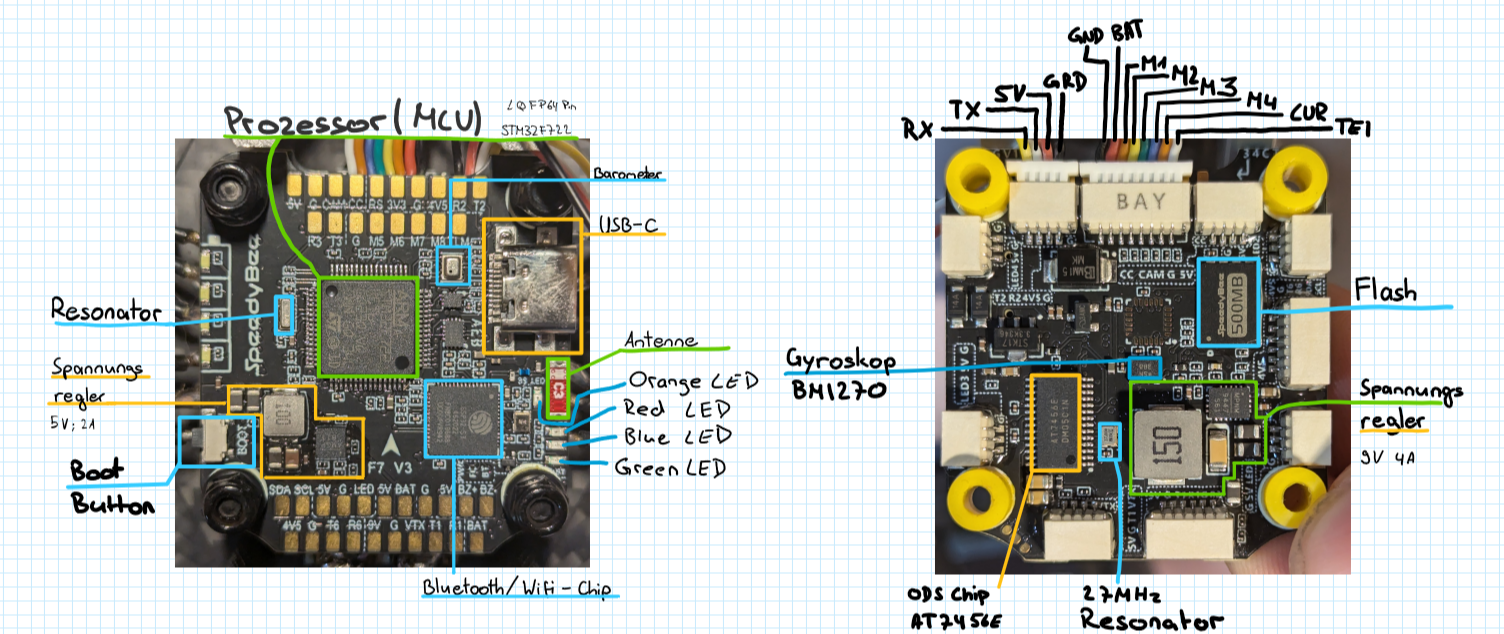
\includegraphics[width=0.635\textheight]{OneNote1&2.png}
\caption{Beschriftung des Prozessors}
\label{fig:OneNote1&2}
\end{figure}
	
Nachdem diese Hürde überwunden war, war der eigentliche Lötprozess und das anschliessende mechanische Zusammenfügen der Bauteile vergleichsweise unkompliziert.

Bei einigen später durchgeführten Tests, stürzte unsere Drohne mehrmals ab und die Propeller brachen. Die Schwierigkeit beim Zusammenbau war sehr unterschiedlich. Am schwierigsten war es, als durch einen Unfall die Verbindung des Motorenkabels, des Stromzufuhrkabels sowie des Kondensators gelöst wurde. Diese Lötstellen mussten zuerst gereinigt und danach neu gelötet werden. Beim Motorenkabel war dies kein Problem. Beim Stromkabel und dem Kondensator hatte man jedoch nur eingeschränkten Zugang, und dazu kam, dass sich die Lötstelle nicht richtig säubern liess. Wir haben versucht sie mit Alkohol zu säubern und abzuschleifen, doch alles vergebens. Die Stromzufuhr und der Kondensator hielten nicht. Nach den Hilfsversuchen von zwei Lehrern sah die Situation immer noch nicht besser aus, weshalb man sich entschloss, professionelle Hilfe in Anspruch zu nehmen. Es wurde Kontakt zum Sponsor der Maturaarbeit, dem Altersheim Abendruh \cite{Altersheim}, aufgenommen, um nach einem Elektriker zu fragen. Dieser reparierte die Drohne im Handumdrehen, und sie funktionierte wieder einwandfrei.

\section{Fazit}

Zusammenfassend lässt sich feststellen, dass der Bau der Drohne ein gewisses Fingerspitzengefühl braucht, ansonsten vergleichsweise leicht durchführbar ist. Trotz anfänglicher Herausforderungen bei der Identifizierung der Teile und korrekten Lötpunkte konnten durch eine sorgfältige Planung alle Probleme gelöst werden.
Die gewählten Bauteile haben sich, wie vorausgesehen, als gut kompatibel erwiesen. Insgesamt erfüllt die Drohne die gestellten Anforderungen und ist bereit für weitere Tests und den praktischen Einsatz.








